\begin{figure}[H]
    \centering
    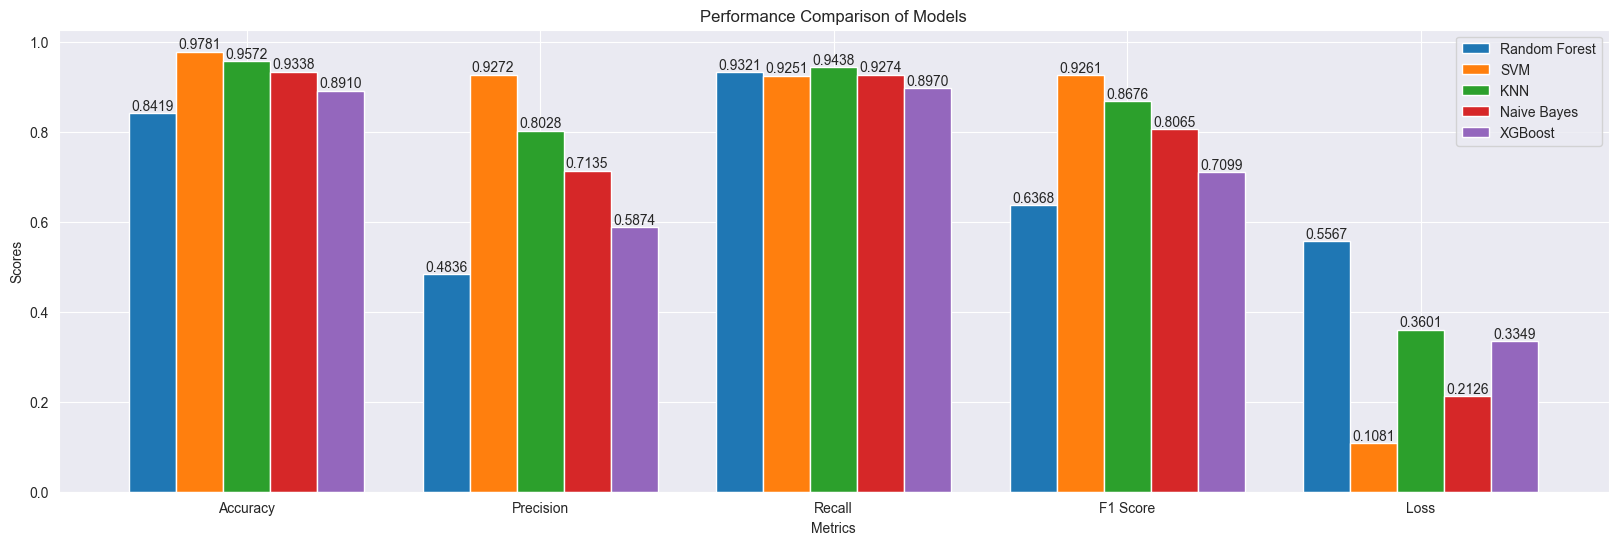
\includegraphics[width=\linewidth]{images/models_performance_validating}
    \caption{}
    \label{fig:models_performance_validating}
\end{figure}

\begin{itemize}
    \item \textbf{General Trend Compared to Previous (Assumed Training) Data:}
    \begin{itemize}
        \item A significant drop in performance is observed across all models and most metrics (Accuracy, Precision, F1 Score) when comparing to the previously analyzed dataset (which had near-perfect scores). Recall scores are somewhat more varied, with some models maintaining high recall. Loss values have generally increased.
        \item This substantial decrease strongly suggests that the models may have overfit to the previous dataset, or that this new dataset presents a more challenging distribution, is inherently more complex, or has a different class balance. The previous high scores might not have been indicative of true generalization capability.
    \end{itemize}

    \item \textbf{Accuracy:}
    \begin{itemize}
        \item SVM exhibits the highest accuracy (0.9781) on this dataset, maintaining strong performance, though lower than its previously observed near-perfect score.
        \item KNN follows with a good accuracy of 0.9572.
        \item Naive Bayes (0.9338), XGBoost (0.8910), and Random Forest (0.8419) show a more considerable drop in accuracy. Random Forest's accuracy is now the lowest.
    \end{itemize}

    \item \textbf{Precision:}
    \begin{itemize}
        \item SVM leads with the highest precision (0.9272), a significant decrease from its previous perfect score but still the best.
        \item KNN (0.8028) and Naive Bayes (0.7135) maintain moderate precision.
        \item Random Forest (0.4836) and XGBoost (0.5874) show a very sharp decline in precision, indicating a large increase in false positives on this new dataset. This is a major change from their previously high precision.
    \end{itemize}

    \item \textbf{Recall:}
    \begin{itemize}
        \item KNN achieves the highest recall (0.9438) on this dataset.
        \item Random Forest (0.9321), SVM (0.9251), and Naive Bayes (0.9274) also maintain high recall scores, suggesting they are still effective at identifying positive instances.
        \item XGBoost's recall (0.8970) is also high, though slightly lower than the others in this group.
        \item The high recall for models like RF and KNN, despite lower precision, suggests they are casting a wide net, correctly identifying positives but also incorrectly flagging many negatives.
    \end{itemize}

    \item \textbf{F1 Score:}
    \begin{itemize}
        \item SVM has the highest F1 Score (0.9261), indicating the best balance between its high precision and high recall on this dataset.
        \item KNN (0.8676) also shows a good F1 Score.
        \item Naive Bayes (0.8065), XGBoost (0.7099), and Random Forest (0.6368) have lower F1 Scores, primarily impacted by their significant drop in precision (for RF and XGBoost) or a less optimal balance.
    \end{itemize}

    \item \textbf{Loss:}
    \begin{itemize}
        \item SVM maintains the lowest loss (0.1081), consistent with its strong performance across other metrics, though this loss is much higher than its previous near-zero loss.
        \item Naive Bayes (0.2126) has the next lowest loss.
        \item XGBoost (0.3349) and KNN (0.3601) have moderate loss values.
        \item Random Forest exhibits the highest loss (0.5567) on this dataset, correlating with its lower precision and accuracy.
    \end{itemize}

    \item \textbf{Overall Observations and Key Changes from Previous Dataset:}
    \begin{itemize}
        \item SVM demonstrates the most robust generalization, leading in Accuracy, Precision, F1 Score, and having the lowest Loss on this new, more challenging dataset. While its scores have decreased from the (assumed) training set, the drop is less severe compared to some other models.
        \item Random Forest and XGBoost show a dramatic decrease in Precision, leading to significantly lower F1 Scores. This suggests they might be particularly sensitive to changes in data distribution or may have learned overly specific patterns from the previous dataset. Their high recall now comes at the cost of many false positives.
        \item KNN, while having the highest loss previously, now shows a more competitive F1 score due to maintaining high recall and moderate precision. Its loss is still relatively high but not the outlier it was.
        \item Naive Bayes maintains relatively stable performance, with its precision dropping but recall remaining high.
        \item The major changes in performance indicate that this new dataset likely differs significantly from the one previously evaluated (assumed to be training/easier validation). This could be due to different underlying data characteristics, a shift in the data distribution (concept drift), or the presence of more noise or outliers. The previous near-perfect scores for some models were likely not representative of real-world generalization.
    \end{itemize}
\end{itemize}

\begin{table}[H]
    \centering
    \caption{Model Performance Comparison (Based on Validating Dataset)}
    \setlength{\tabcolsep}{3pt}
    \renewcommand{\arraystretch}{1.2}
    \resizebox{240pt}{!}{
        \begin{tabular}{|p{2.8cm}|p{2.8cm}|}
            \hline
            \textbf{Model} & \textbf{Key Analysis}                                                                           \\
            \hline
            Random Forest  & Lowest Acc. Very low Prec., high Recall (many FPs). Highest Loss. Significant performance drop. \\
            \hline
            SVM            & Best performer overall. Highest Acc, Prec, F1. Lowest Loss. Most robust generalization.         \\
            \hline
            KNN            & Good Acc. Highest Recall. Moderate Prec \& F1. High Loss. Performance drop but recall strong.   \\
            \hline
            Naive Bayes    & Moderate Acc                            \& Prec. High Recall. Second lowest Loss. Performance drop but relatively stable.   \\
            \hline
            XGBoost        & Moderate Acc. Low Prec., high Recall (many FPs). Moderate Loss. Significant drop in Prec/F1.    \\
            \hline
        \end{tabular}
    }
    \label{tab:model_performance_new_barchart}
\end{table}